%%%%%%%%%%%%
%
% $Autor: Wings $
% $Datum: 2019-03-05 08:03:15Z $
% $Pfad: TemplateSensor $
% $Version: 4250 $
% !TeX spellcheck = en_GB/de_DE
% !TeX encoding = utf8
% !TeX root = filename 
% !TeX TXS-program:bibliography = txs:///biber
%
%%%%%%%%%%%%

% Structure
\chapter{Spannungsversorgung - AC/DC Wandler}

In Mikrokontroller-Anwendungen ist eine stabile Gleichspannungsquelle erforderlich, um Sensoren, Aktoren sowie den Mikrokontroller selbst zuverlässig betreiben zu können. Üblicherweise werden Spannungswandler eingesetzt, die eine Ausgangsspannung von 3,3~V oder 5~V liefern.
Wird das System über einen Computer oder ein USB-Netzteil betrieben, erfolgt die Spannungsversorgung meist über den USB-Port. Der Arduino verfügt jedoch auch über spezielle Pins, über die eine externe Spannung eingespeist und durch einen integrierten Spannungsregler geführt werden kann. Dadurch lässt sich ein AC/DC-Wandler direkt mit dem Spannungseingang des Boards verbinden -- der USB-Port bleibt frei, und der Aufbau der Schaltung kann kompakter gestaltet werden.
In diesem Projekt wird ein AC/DC-Wandler verwendet, der Netzspannungen im Bereich von 80 bis 240~V AC in eine stabile 5~V DC-Spannung umwandelt.

%\section{General}


\section{Eingesetzter Spannungswandler}

Für diese Anwendung wird der AC/DC-Wandler IRM-15-5 von der Firma Mean Well eingesetzt, der eine Eingangsspannung von 85 - 305 VAC und eine Ausgangsspannung von 5 VDC bei max. 2 A bereitstellt. Er zeichnet sich durch seine hohe Kompatibilität, zuverlässigen Schutzmechanismen und einen guten Wirkungsgrad aus. Der Wandler wird dauerhaft an die 230 V Netzspannung angeschlossen, um das Arduino sowie die daran angeschlossenen Sensoren und Aktoren zu betreiben. Dieser Sensor erfordert eine Montage auf der Platine (THT – Through-Hole Technology).

\begin{center}
	\begin{tikzpicture}
		\powerSupply
	\end{tikzpicture}
	\captionof{figure}{15W AC/DC PCB Wandler}
\end{center}

\begin{center}
	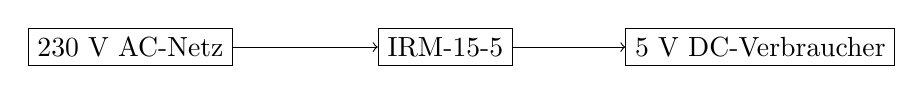
\begin{tikzpicture}[node distance=2cm, auto]
		\node (netz) [draw, rectangle] {230 V AC-Netz};
		\node (wandler) [right of=netz, draw, rectangle, node distance=4cm] {IRM-15-5};
		\node (last) [right of=wandler, draw, rectangle, node distance=4cm] {5 V DC-Verbraucher};
		
		\draw[->] (netz) -- (wandler);
		\draw[->] (wandler) -- (last);
	\end{tikzpicture}
	\captionof{figure}{Blockschaltbild der Spannungsversorgung}
\end{center}

\section{Spezifikation}
		\begin{table}[H]
		\centering
		\begin{tabular}{|l|l|}
			\hline
			\textbf{Eigenschaft} & \textbf{Wert} \\
			\hline
			Eingangsspannung & 85 - 305 VAC / 120 - 430 VDC \\
			\hline
			Frequenzbereich & 47 - 440Hz \\
			\hline
			Ausgangsspannung & 5 VDC \\
			\hline
			Ausgangsstrom & 0 - 3 A \\
			\hline
			Leistung & 15 W \\
			\hline
			Wirkungsgrad & 78 \% \\
			\hline
			Betriebstemperaturbereich & -30 ... +70  $^{\circ}$Celsius \\
			\hline
			Lagerungstemperaturbereich & -40 ... +85  $^{\circ}$Celsius \\
			\hline
			Einschaltstrom & max. 40 A bei 230 VAC\\
			\hline
			Abmessungen (LxBxH) & 52.4 x 27.2 x 24 mm \\
			\hline
			Gewicht & 0,05 kg \\
			\hline
		\end{tabular}
		\caption{Technische Spezifikationen WM AC/DC IRM-15-5 Wandlers. \cite{Wangj:2019}}
	\end{table}

\section{Funktionsprinzip}
		
	Ein AC/DC-Wandler, auch als Netzteil bekannt, dient der Umwandlung von Wechselspannung (AC) aus dem Stromnetz in eine stabile Gleichspannung (DC), die für elektronische Schaltungen und Mikrocontroller erforderlich ist. Das Funktionsprinzip lässt sich in mehrere Stufen unterteilen:
	
	\begin{enumerate}
		\item \textbf{Eingangsfilterung:} Zur Unterdrückung von Netzstörungen und elektromagnetischen Interferenzen (EMI) wird die Eingangsspannung zunächst durch Filterelemente (z.\,B. Drosseln und Kondensatoren) geglättet.
		\item \textbf{Gleichrichtung:} Mithilfe einer Gleichrichterschaltung, meist in Form eines Brückengleichrichters, wird die Wechselspannung in eine pulsierende Gleichspannung umgewandelt.
		\item \textbf{Glättung:} Ein Elektrolytkondensator glättet die pulsierende Gleichspannung und reduziert Spannungsschwankungen.
		\item \textbf{Spannungsregelung:} Ein Spannungsregler (linear oder schaltend) stabilisiert die Ausgangsspannung auf konstante 5\,V.
		\item \textbf{Schutzfunktionen:} Der Wandler verfügt über integrierte Schutzschaltungen, die bei Überstrom, Kurzschluss oder Übertemperatur eingreifen und das System vor Schäden bewahren.
	\end{enumerate}
		Durch diese mehrstufige Umwandlung wird eine zuverlässige und stabile Versorgungsspannung bereitgestellt, die den sicheren Betrieb von Mikrocontrollern und angeschlossenen Komponenten gewährleistet.
				
\subsection{Blockdiagramm eines AC/DC Wandlers}
\begin{center}
	\begin{tikzpicture}[scale=0.7]
		\powerSupplyCircuit
	\end{tikzpicture}
	\captionof{figure}{AC/DC Wandler - Blockdiagramm\cite{Wangj:2019}}
\end{center}


\subsection{Transformator}
	In Niederspannungsschaltungen übernimmt dieses Bauteil mehrere zentrale Aufgaben:
	\begin{itemize}
		\item \textbf{Spannungsreduzierung:} Es senkt die Netzspannung auf ein niedrigeres Niveau, das für elektronische Komponenten geeignet ist.
		\item \textbf{Galvanische Trennung:} Der Ausgangskreis wird vom Eingangskreis elektrisch isoliert, was die Sicherheit erhöht und das System vor Überspannungen schützt.
		\item \textbf{Reduktion elektromagnetischer Störungen (EMI):} Störungen aus dem Stromnetz werden wirksam unterdrückt.
	\end{itemize}
	
	Der Transformator wandelt Wechselspannungen durch ein bestimmtes Windungsverhältnis zwischen Primär- und Sekundärwicklung. Dabei kann die Spannung gezielt erhöht oder verringert werden, wobei sich der Strom entsprechend verändert\cite{Rolink:2025}. 
	Die grundlegende Formel für ein ideales Modell lautet:
	
	
	\[
	\frac{U_1}{U_2} = \frac{N_1}{N_2}
	\]
	
	wobei:
	\begin{itemize}
		\item \(U_1\): Spannung auf der Primärseite des Transformators
		\item \(U_2\): Spannung auf der Sekundärseite des Transformators
		\item \(N_1\): Anzahl der Windungen auf der Primärseite
		\item \(N_2\): Anzahl der Windungen auf der Sekundärseite
	\end{itemize}
	
	Für einen idealen Transformator, bei dem keine Verluste auftreten, gilt zusätzlich:
	
	\[
	P_1 = P_2 \quad \Rightarrow \quad U_1 \cdot I_1 = U_2 \cdot I_2
	\]
	
	wobei:
	\begin{itemize}
		\item \(I_1\): Strom auf der Primärseite
		\item \(I_2\): Strom auf der Sekundärseite
		\item \(P_1\), \(P_2\): Leistung auf der Primär- bzw. Sekundärseite
	\end{itemize}
	
	Somit kann beobachtet werden, dass bei steigender Spannung der Strom entsprechend sinkt:
	
	\[
	\frac{U_1}{U_2} = \frac{N_1}{N_2} = \frac{I_2}{I_1}
	\]
	
	
	\subsubsection{Effektivität eines Transformators}
	Die Effektivität eines Transformators beschreibt das Verhältnis der abgegebenen Leistung zur zugeführten Leistung. In einem idealen Transformator würde die gesamte zugeführte Energie in Ausgangsleistung umgewandelt, jedoch treten immer Verluste (meistens als Wärme) auf, wodurch die Effektivität nie 100\% beträgt.
	Die Effektivität eines Transformators beschreibt die folgende Formel:
	\[
	\eta = \frac{P_{\text{ab}}}{P_{\text{zu}}} \cdot 100
	\]
	wobei:
	\begin{itemize}
		\item \(P_{\text{ab}}\) : die abgegebene Leistung ist
		\item \(P_{\text{zu}}\) : die zugeführte Leistung ist
	\end{itemize}
	
	Diese Formel zeigt, dass die Effektivität eines Transformators als Prozentsatz des Anteils der zugeführten Energie berechnet wird, der effektiv in nutzbare Ausgangsleistung umgewandelt wird.
	
	\subsubsection{Verluste im Transformator}
	Es gibt verschiedene Arten von Verlusten, die die Effektivität rinrs Transformators negativ beeinflussen. Zu den wichtigesten gehören:
	\begin{itemize}
		\item \textbf{Kupferverluste:} Diese Verluste entstehen durch den Wiederstand der Wicklungen des Transformators, sowohl auf der Primär- als auch auf der Sekundärseite. Der Wiederstand des Drahts erzeugt Wärme, die zu Verlusten führt. Diese Verluste sind proportional zu STromstärke und dem Wiederstand der Wicklungen und lassen sich durch folgende Gleichung berechnen:
		\[P_{\textbf{Kupfer}} = I^2 \cdot R\] wobei \(I\) die Stromstärke und \(R\) der Wiederstand der Wicklungen ist.
		
		\item \textbf{Eisenverluste (Kernverluste):} Diese Verluste treten im Eisenkern des Transformators auf, wenn der magnetische Fluss, der durch den Kern flie{\ss}t, ständig seine Richtung ändert. Die Eisenverluste setzen sich aus zwei Hauptkomponenten zusammen:
		\begin{itemize}
			\item \textbf{Hystereseverluste:} Diese Verluste entstehen durch die Umkehrung der Magnetisierung im Kernmaterial und sind proportional zur Frequenz und zum Material des Kerns.
			\item \textbf{Wirbelstromverluste:} Diese Verluste entstehen durch die induzierten Ströme im Kernmaterial aufgrund des sich ändernden Magnetfeldes. Sie sind ebenfalls frequenzabhängig und werden durch den Widerstand des Kernmaterials beeinflusst.
		\end{itemize}
		
		\item \textbf{Dielektrische Verluste:} Diese Verluste entstehen durch die Isolierung des Transformators. Sie sind in der Regel geringer als die Kupfer- und Eisenverluste, können jedoch bei sehr hohen Spannungen oder Frequenzen eine bedeutende Rolle spielen.
		
		\item \textbf{Mechanische Verluste:} Diese Verluste entstehen durch mechanische Vibrationen des Transformators, die durch die magnetische Wechselwirkung zwischen den Wicklungen und dem Eisenkern verursacht werden. Obwohl mechanische Verluste normalerweise gering sind, können sie bei gro{\ss}en Transformatoren oder hohen Frequenzen bedeutender werden.
	\end{itemize}
	

\section{Schutzvorrichtungen}
	AC/DC-Wandler IRM-15-5 verfügt über viele Schutzvorrichtungen und Sicherheitsmechanismen, die den sicheren Betrieb des Gerätz gewährleisten:
	\subsection{Überlastungsschutz}
	Sobald eine Überlastung auftritt, schaltet der Wandler automatisch ab, um die Beschädigung anderer Komponenten zu vermeiden. Sobald die fehlerhafte Bedingung behoben wurde, wird das Modul automatisch wiederhergestellt. Der Schutzbereich dieses Modells liegt zwischen 115\,\% und 260\,\% der Nennleistung des Ausgangs.
	\subsection{Überspannungsschutz}
	Sobald eine Überspannung auftritt, wird der Ausgang durch eine Zenerdiode auf einen sicheren Wert begrentzt. Der Schutzbereich dieses Models liegt zwischen 5{,}75\,V und 6{,}75\,V, wie im Datenblatt angegeben.

\section{Montage}
Der AC/DC-Wandler IRM-15-5 ist ein THT-Bauelement (Through-Hole Technology) und wird zur Montage durch Bohrungen auf der Leiterplatte gesteckt und anschlie{\ss}end fest verlötet. Diese Befestigungsart sorgt für eine stabile mechanische Verbindung und eignet sich besonders für Anwendungen mit höheren mechanischen Belastungen.

Anschlussbeschreibung:
\begin{itemize}
	\item \textbf{AC/L:} Wechselstrom-Leiter (Phase) - Netzspannungseingang
	\item \textbf{AC/N:} Wechselstrom-Neutralleiter - Netzspannungseingang
	\item \textbf{+V:} Gleichspannungs-Ausgang (positiver Pol)
	\item \textbf{-V:} Gleischspannungs-Ausgang (negativer Pol)
\end{itemize}

Die Gleichspannungsausgänge sollten mit einem 100 \(\mu\)F Kondensator überbrückt werden, um eine bessere Stabilität zu erreichen. Der Wandler soll mit folgenden Pins von Arduino gekoppelt werden:
\begin{itemize}
	\item V+ \(\rightarrow \text{VIN}\)
	\item V- \(\rightarrow \text{GND}\)
\end{itemize}


% schaltung wie anschlie{\ss}en

\section{Spannungserkennung\label{powerSupply:voltageDetection}}
	Es kann überprüft werden, ob die Spannungsquelle funktioniert und eine Spannung liefert. Dazu messen wir die Spannung zwischen dem positiven Pol des AC/DC-Wandlers und dem \texttt{VIN}-Pin des Arduino.
	
	Da die Referenzspannung des Boards bei $3{,}3\,\mathrm{V}$ liegt, muss die Eingangsspannung (\(5\,V\))auf ein sicheres Niveau reduziert werden. Hierzu wird ein Spannungsteiler\ref{voltageDivider} verwendet.
	
	Es muss beachtet werden, dass der Arduino ohne eine geeignete Spannungsversorgung nicht funktionieren kann – das hei{\ss}t, wenn keine Backup-Stromquelle vorhanden ist, schaltet sich der Arduino sofort aus, sobald die Spannung vom AC/DC-Wandler ausfällt. Deswegen um diese Anwendung zu Testen, brauchen wir eine Backup-Stromquelle.
	
	Dabei ist jedoch besonders wichtig, dass \textbf{nicht mehrere Spannungsquellen gleichzeitig} verwendet werden dürfen – beispielsweise dürfen USB und der \texttt{VIN}-Pin nicht gleichzeitig angeschlossen sein, da dies zu Schäden an der internen Stromverteilung des Arduino führen kann.
	
	Erlaubte Konfigurationen sind jedoch:
	\begin{itemize}
		\item \textbf{USB + Akku}
		\item \textbf{VIN + Akku}
	\end{itemize}
	
	\subsection{Spannungsteiler mit zwei ohmisschen Widerständen - Prinzip\label{voltageDivider}}
	Ein Spannungsteiler besteht meistens aus zwei Widerständen.
		\begin{center}
			\begin{circuitikz}[european]
				%\tikzset{voltage dir = RP}
				\draw (0,5) to [V, v_=$U_{in}$, i<=$I_0$]  (0,0); 
				\draw(0,5) -- (3, 5)
				to[R, l_=$R_1$, v^=$U_1$, i>_=$I_1$] (3, 2.5)
				to[R, l_=$R_2$, *-*, v^=$U_2$, i>_=$I_2$] (3, 0) -- (0,0);
				\draw (3,2.5) -- ++(1.5,0) node[ocirc]{};
				\draw (3,0) -- ++(1.5,0) node[ocirc]{};
				\draw (4.5,2.5) to[open, v^=$U_{out}$, voltage=straight] (4.5,0);
			\end{circuitikz}
			\captionof{figure}{Widerstands-Spannungsteiler}
		\end{center}
	
	Zur Berechnung von \(U_2\) wird zunächst der Gesamtwiderstand \(R_{ges}\) benötigt. In einer Reihenschaltung berechnet er sich wie folgt:
	\begin{equation}
		R_{ges} = R_1 + R_2
	\end{equation}

	Die Gesamtspannung sowie die Werte \(R_1\) und \(R_2\) sind bekannt. Daher lässt sich gemä{\ss} dem ohmschen Gesetz der Strom \(I\) bestimmen:
	\begin{equation}
		I_0 = \frac{U_{in}}{R_{ges}} = \frac{U_{in}}{R_1 + R_2}
	\end{equation}
	Der Strom ist in einer Reihenschaltung in allen Bauteilen gleich:
	\begin{equation}
		I_0 = I_1 = I_2
	\end{equation}

	Somit ergibt sich die gesuchte Spannung \(U_2\):
	\begin{equation}
		U_2 = I_0 \cdot R_2
	\end{equation}

	Durch Einsetzen ergibt sich:
	\begin{equation}
		U_2 = \frac{U_{in}}{R_{ges}} \cdot R_2  = U_{in} \cdot \frac{R_2}{R_1 + R_2}
		\label{voltageDivider:formula}
	\end{equation}

	
	Die Spannung \(U_2\) ist also proportional zur Eingangsspannung \(U_\text{in}\). Durch Anwenden der Formel
	\begin{equation}
		U_\text{in} = \frac{U_2 \cdot R_\text{ges}}{R_2}
	\end{equation}

	kann die Eingangsspannung \(U_in\) bestimmt werden, wobei \(U_2\), \(R_2\) und \(R_\text{ges}\) bekannt sein müssen.
	
	
	\subsection{Beispiel\label{voltageDivider:example}}
	Angenommen, unsere Spannungsquelle liefert \(5\,V\). Die Referenzspannung des Arduinos beträgt jedoch \(3,3\,V\). Wir müssen also die zu messende Spannung so anpassen, dass sie im Bereich von \(0\,V\) - \(3,3\,V\) liegt, dabei aber die tatsächliche Spannung korrekt wiederspiegelt. 
	
	Nehmen wir an, dass unsere Spannungsquelle eine abweichung bis zu 2,5\% aufweist. Diese Abweichung müssen wir berücksichtigen und auf den zulässigen Bereich abbilden. Das ergibt einen möglichen Spannunsbereich von:
	\[
	\pm 2{,}5\,\% \text{ von } 5{,}0\,\mathrm{V} = [4{,}875\,\mathrm{V},\,5{,}125\,\mathrm{V}]
	\]
	
	
	Wir setzen die bisher bekannte Werte unter Berücksichtigung der neuen maximalen Spannung von \(5,125\,V\) in die Formel \ref{voltageDivider:formula} ein:
	\begin{equation}
		3,3\,V = \frac{5,125\,V}{R_1 + R_2} \cdot R_2 \iff 3,3\,V = 5,125\,V \cdot \frac{R_2}{R_1 + R_2}
	\end{equation}
	Hier sieht man, dass noch das Verhältnis \(R_2\) zu \(R_{ges}\) fehlt.
	Die Schaltung soll hochohmig sein, um den Stromfluss möglichst gering zu halten. Es kommen daher gro{\ss}e Widerstände in Frage (mehrere Kiloohm bis Megaohm). Da die Ströme beim Arduino relativ klein sind, bleiben wir bei den kleineren Werten in diesem Bereich.
	Aus der Formel \ref{voltageDivider:formula} ergibt sich:
	\begin{equation}
		\frac{U_2}{U_{ges}} = \frac{R_2}{R_{ges}}
	\end{equation}
	Wir benötigen also Widerstände mit einem ähnlichen Verhältnis von \(R_2\) zu \(R_{ges}\) wie die Spannungen, also \(\frac{3,3\,V}{5,125\,V} \approx 0,64\,V\).
	Wir entscheiden uns für einen Widerstand \(R_2 = 100k\Omega\). Nun berechnen wir \(R_1\):
	\[
		\frac{U_2}{U_{ges}} = \frac{R_2}{R_{ges}} \iff \frac{3,3\,V}{5,125\,V} = \frac{100k\Omega}{R_1 + 100k\Omega} \rightarrow R_1 \approx 55,3k\Omega
	\]
	Aus dieser Berechnung folgt: Wenn \(R_2 = 100\,k\Omega\) , dann beträgt \(R_1 = 55,3\,k\Omega\). Da es keinen genormten Widerstand mit exakt diesem Wert gibt, wählen wir den nächstgrö{\ss}eren verfügbaren Wert, also \(56\,k\Omega\).
	
	Die gewählten Werte lauten:
	\begin{itemize}
		\item \(U_{in} = 5\,V \) 
		\item \(U_{in_{max}} = 5,125\,V \)
		\item \(R_{1} = 56\,k\Omega \)
		\item  \(R_{2} = 100\,k\Omega \)
		\item \(U_{2}\): \[U_{2} = 5\,V \cdot \frac{100\,k\Omega}{156\,k\Omega}\]
		\item \(U_{2_{max}} = 5,125\,V \cdot \frac{100\,k\Omega}{156\,k\Omega} \approx 3,28\,V\)
	\end{itemize}
	
	Nach Einsicht in das Angebot unseres Lieferanten \href{https://www.reichelt.de/de/de/}{Reichelt.de} wurde jedoch festgestellt, dass der ursprünglich vorgesehene 56-k\(\Omega\)-Widerstand (SMD, Bauform 1206) unsere Anforderungen aufgrund seiner zu gro{\ss}en Toleranz nicht erfüllt.
	
	Um möglichst nah an den berechneten Parametern zu bleiben, wurde ein alternativer Widerstand mit ähnlichem Wert ausgewählt. Dabei fiel die Wahl auf einen 62-k\(\Omega\)-\href{https://www.reichelt.de/de/de/shop/produkt/smd-widerstand\_1206\_62\_kohm\_250\_mw\_0\_1\_-377375}{Widerstand} der Marke Panasonic.

	Die neu berechneten Werte lauten:
	\begin{itemize}
		\item \(U_{in} = 5\,V \) 
		\item \(U_{in_{max}} = 5,125\,V \)
		\item \(R_{1} = 62\,k\Omega \)
		\item  \(R_{2} = 100\,k\Omega \)
		\item \(U_{2}\): \[U_{2} = 5\,V \cdot \frac{100\,k\Omega}{162\,k\Omega}\]
		\item \(U_{2_{max}} = 5,125\,V \cdot \frac{100\,k\Omega}{162\,k\Omega} \approx 3,16\,V\)
	\end{itemize}
	%\Mynote{Widerstabd für die Platine}
	
	\subsubsection{Schaltbild}
		\begin{center}
			\begin{circuitikz}[european]
				\draw (6,0) node[ocirc, label=right:GND]{}-- (0,0) to [V, v<=$U_{5V}$]  (0,2) -- (1,2) node[circ](A){} -- (6,2) node[ocirc, label=right:\(VIN_{Arduino}\)]{}; 
				\draw (A) -- ++(0,1) to[R, l=\(R_{62k\Omega}\)] ++(2,0) node[circ](B){} to[R, l=\(R_{100k\Omega}\)] (6,3) node[ocirc, label=right:GND]{};
				\draw (B) -- ++(0,1) -- (6,4) node[ocirc, label=right:\(analogPin_{Arduino}\)]{} node[right]{};
				\draw (6,2) to[open, v^=$U_{5V}$, voltage=straight] (6,0);
				\draw (6,4) to[open, v^=$U_{mess}$, voltage=straight] (6,3);
			\end{circuitikz}
			\captionof{figure}{Spannungsteiler zur Ermittlung der Akkuspannung}
		\end{center}
		%\Mynote{Schiebe Umess}	
		
	\subsubsection{Code\label{powerSupply:codeExample}}
	{
		\captionof{code}{Spannung auslesen}
		\ArduinoExternal{}{../../Code/MKRWAN1310/PowerSupply/checkCurrentVoltage.cpp}
	}
	
\section{Überwachung der Eingangsspannung}

Wie oben in \nameref{powerSupply:voltageDetection} beschrieben, kann ein Mechanismus zur Erkennung der 5~V-Spannung des AC/DC-Wandlers aufgebaut werden. Dafür muss der Arduino jedoch über einen Akku als ``Backup-Spannungsquelle'' verfügen.
	
	Der Mechanismus ist einfach: Es wird eine Grenzspannung festgelegt. Die Spannung des AC/DC-Wandlers wird mithilfe eines Spannungsteilers gemessen. Fällt die Spannung unter diesen Grenzwert oder fällt ganz aus, wird der Arduino vom Akku versorgt und schaltet die rote LED entsprechend ein. Liegt die gelieferte Spannung oberhalb dieser Grenze, leuchtet die grüne LED.
	
	\subsection{Schaltung}
	\Mynote{mache Tikz Schaltung}
	\subsection{Code}
	{
		\captionof{code}{Überwachung der Spannung aus AC/DC Wandler}
		\ArduinoExternal{}{../../Code/MKRWAN1310/PowerSupply/powerSupplyIndicator.cpp}
	}
	
	
	
